\section{pytorch overview}

\subsection{What is pytorch?}


官方的介绍\url{https://pytorch.org/}: An open source deep learning platform that provides a seamless path from research prototyping to production deployment.

\subsection{pytorch 0.4}

Pytorch 0.4和之前的版本,主要提供的是面向researchers的一个易用的深度学习框架。这个时候的pytorch拥有一个优秀的前端,提供了好用的API、python的无缝支持、动态计算图等等。

然而,pytorch这个时候的版本并不适合于生产环境。这是由于pytorch与python紧密结合,以及动态计算图是imperative的(命令式的,即一步步执行,pytorch并不知道下一步的执行操作是什么,所以难以优化)。所以一般会只用pytorch进行研发,之后再将其转移到适合生产环境的框架中。

一个做法是将pytorch model转换成ONNX(Open Neural Network Exchange),再转换成
caffe2框架。

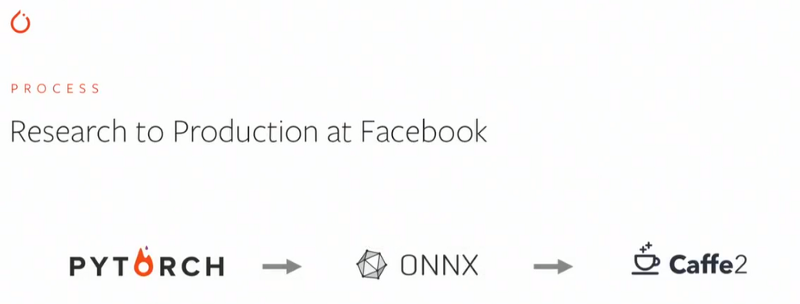
\includegraphics[width=0.8\linewidth]{pytorch/pic/pytorch_to_caffe2.png}

ONNX(Open Neural Network Exchange):深度学习框架中迁移模型的中间表达格式框架。

Caffe2:一个关注性能和多平台支持的深度学习框架。

\subsection{pytorch 0.4 to pytorch 1.0}

pytorch 1.0 做出的一个重大改变是将caffe2和pytorch结合起来,使得开发和生产环境可
以使用同一个框架。

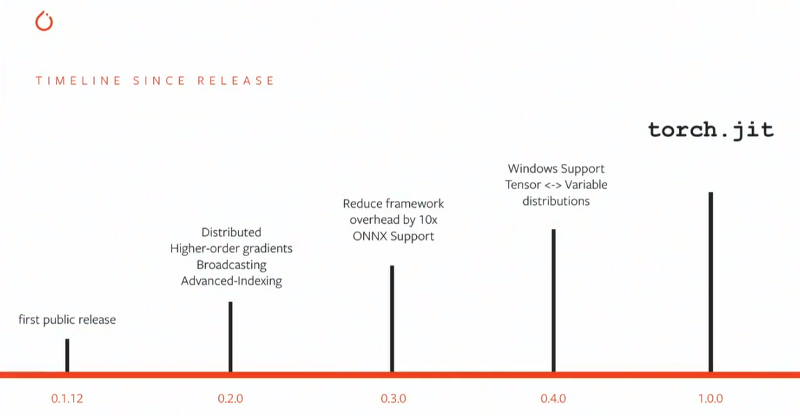
\includegraphics[width=0.8\linewidth]{pytorch/pic/road_to_pytorch_1_0.png}

pytorch 1.0 引入了\texttt{torch.jit}模块。这个模块是一个 just-in-time (JIT) compiler,可以将pytorch model序列化python-free(不需要python)的中间表示。这个模块为了解决两个问题:
\begin{itemize}
  \tightlist
  \item
    将模型和代码分离,使得模型可以在python-free的环境中使用。
  \item
    为了提供更好的性能,命令式的执行使得pytorch难以对模型进行优化,\texttt{torch.jit}模块可以得知整个模型的执行流程从而可以对模型进行优化。
\end{itemize}

现在pytorch就可以使用两种开发模式:Eager Mode(命令式,用于研发)和 Script Mode(使
用\texttt{torch.jit}的torch script 序列化成python-free的中间表示, 用于生产环
境)。

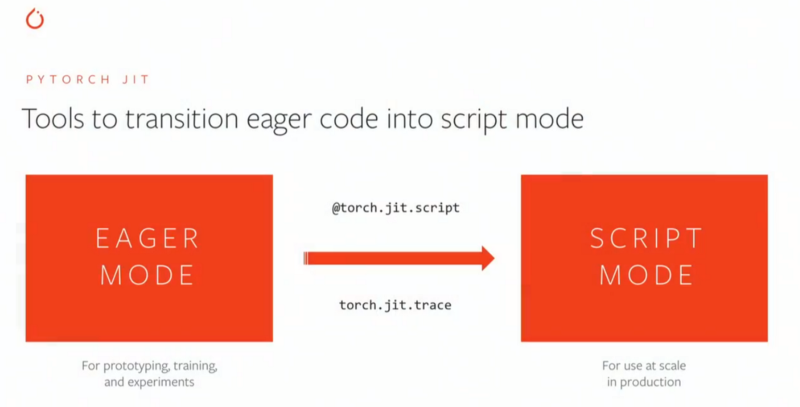
\includegraphics[width=0.8\linewidth]{pytorch/pic/pytorch_mode.png}

\subsection{pytorch 1.0 to 1.1}

PyTorch 1.1 增加了 TensorBoard  支持. JIT 中自定义 RNN 网络, 以及对 JIT 的一些改进.

\href{https://www.tensorflow.org/tensorboard/}{TensorBoard} 是 TensorFLow 的可视
化工具. 支持:
\begin{itemize}
\item
Tracking and visualizing metrics such as loss and accuracy
\item
Visualizing the model graph (ops and layers)
\item
Viewing histograms of weights, biases, or other tensors as they change over time
\item
Projecting embeddings to a lower dimensional space
\item
Displaying images, text, and audio data
\item
Profiling TensorFlow programs
\item
And much more
\end{itemize}

1.1 增加了在 TorchScript(JIT) 中\href{https://pytorch.org/blog/optimizing-cuda-rnn-with-torchscript/}
{自定义 RNN 的支持}, 之前的实现使用一个 fuesd CUDA kernel, 难以修改.

1.1 对JIT还做了如下修改
\begin{itemize}
\item
\textbf{Attributes in ScriptModules}: Assign attributes on a ScriptModule by wrapping them with torch.jit.Attribute . This update supports all types available in TorchScript. After assigning an attribute, PyTorch saves the attribute in a separate archive in the serialized model binary.
\item
\textbf{Dictionary and list support in TorchScript}: Lists and dictionary types behave like Python lists and dictionaries.
\item
\textbf{User-defined classes in TorchScript}
\end{itemize}


\subsection{torch.jit}

\texttt{torch.jit}提供了两种模式转换python code成中间表示。

一种是Tracing mode,可以将现存的Eager Mode的python models序列化成中间表示而无需对代码进行过多的改造。trace不会管代码的结构,它只会记录所有它遇到的操作。所以tracing mode比较适合于没有条件分支的模型,因为trace不会记录分支判断,它只记录操作。所以即使data值改变使得条件分支发生了变化,trace还是会走上一次的分支,因为上一次就是这么操作的。而loop循环也会被展开,所以如果循环次数与data值相关,那么不应该使用tracing mode。

\begin{lstlisting}
  # This will run your nn.Module or regular Python function with the example
  # input that you provided. The returned callable can be used to re-execute
  # all operations that happened during the example run, but it will no longer
  # use the Python interpreter.
  from torch.jit import trace
  traced_model = trace(model, example_input=input)
  traced_fn = trace(fn, example_input=input)

  # The training loop doesn't change. Traced model behaves exactly like an
  # nn.Module, except that you can't edit what it does or change its attributes.
  # Think of it as a "frozen module".
  for input, target in data_loader:
      loss = loss_fn(traced_model(input), target)
\end{lstlisting}

另一种是script mode,在python函数上使用\texttt{@script} decorator(装饰器)。这个
decorator可以将python函数转换成高效的c++ runtime。这样就可以记录条件分支和循环
了。这个decorator,或者说Torch script使用的是python的一个子集。

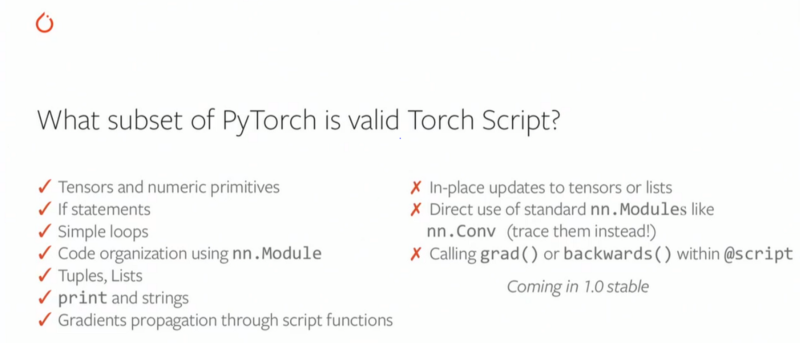
\includegraphics[width=0.8\linewidth]{pytorch/pic/torch_script.png}

\begin{lstlisting}
from torch.jit import script

@script
def rnn_loop(x):
    hidden = None
    for x_t in x.split(1):
        x, hidden = model(x, hidden)
    return x
\end{lstlisting}

\subsection{参考文章}

\begin{itemize}
\tightlist
\item
  pytorch官方blog:\url{https://pytorch.org/blog/the-road-to-1_0/}
\item
  torch.jit:\url{https://pytorch.org/docs/stable/jit.html}
\item
  一篇介绍pytorch的blog:
  \url{https://towardsdatascience.com/a-first-look-at-pytorch-1-0-8d3cce20b3ee}
\item Pytorch 1.1 的介绍: \href{https://jaxenter.com/pytorch-1-1-158332.html}
{PyTorch 1.1 improves JIT compilation and offers TensorBoard support}
\end{itemize}
